\chapter{Introduction}
\label{ch:intro}

\section{Motivation}
In a lecture with 40 or 50 students the air in the classroom gets bad quickly. The reason is the \cotwo{} that
we breathe out. Outdoor air has about 400~ppm of \cotwo{}, and in a full room without fresh air the value can
go above 1000~ppm within one lecture. In a study people made clearly worse decisions at 1000~ppm than at 600~ppm
\citep{satish2012}, and the German Umweltbundesamt rates values below 1000~ppm as harmless and values above
2000~ppm as not acceptable \citep{uba2008}. We cannot see or smell \cotwo{}, so normally nobody in the room
notices it.

In our classrooms the only way to get fresh air is to open the windows. In winter this is a problem, because
the warm air goes out and the room has to be heated again. If we knew how the \cotwo{} will develop in the
next minutes, we could open the windows at the right time and close them again when the air is good. For this
we need a model that predicts the \cotwo{} in the room. In this thesis I only predict the \cotwo{}. The
temperature and the heating energy are not part of the model.

The airflow in a room can be calculated with computational fluid dynamics (CFD), but one simulation takes
many hours, so it cannot be used while a lecture is running. \citet{bian2025} solved this for a classroom with
ceiling vents. They ran many CFD simulations before, trained a neural network on the results, and this
network gives a prediction in less than a second.

\section{Goal of this thesis}
The goal of this thesis is to use the method of \citet{bian2025} for classroom 1-130 of our university. This
room has no ceiling vents. It is ventilated through 8 windows and 2 doors. A wireless sensor network (WSN) is
being installed in the room, and later the model should work with the data of these sensors. I use only
open-source software, with OpenFOAM for the simulations instead of ANSYS Fluent.

\section{Approach}
I run OpenFOAM simulations of the room and use this data to train the GNOT model. \fref{fig:pipeline} shows
the steps. One simulation belongs to one window scenario, which says which windows are open and how fast the
air comes in. OpenFOAM calculates the airflow, and my own \cotwo{} solver calculates from this airflow how the
\cotwo{} of the people spreads in the room over 30~minutes. The model is trained on these \cotwo{} maps. It
gets the \cotwo{} of the last 6~minutes at 1.6~m height, the window speeds and the number of people, and it
predicts the \cotwo{} of the next 3~minutes. I use 1.6~m, which is about the head height of a standing person. The \cotwo{} is
stored for the whole room, so another height can be used later without new simulations.

\begin{figure}[h]
  \centering
  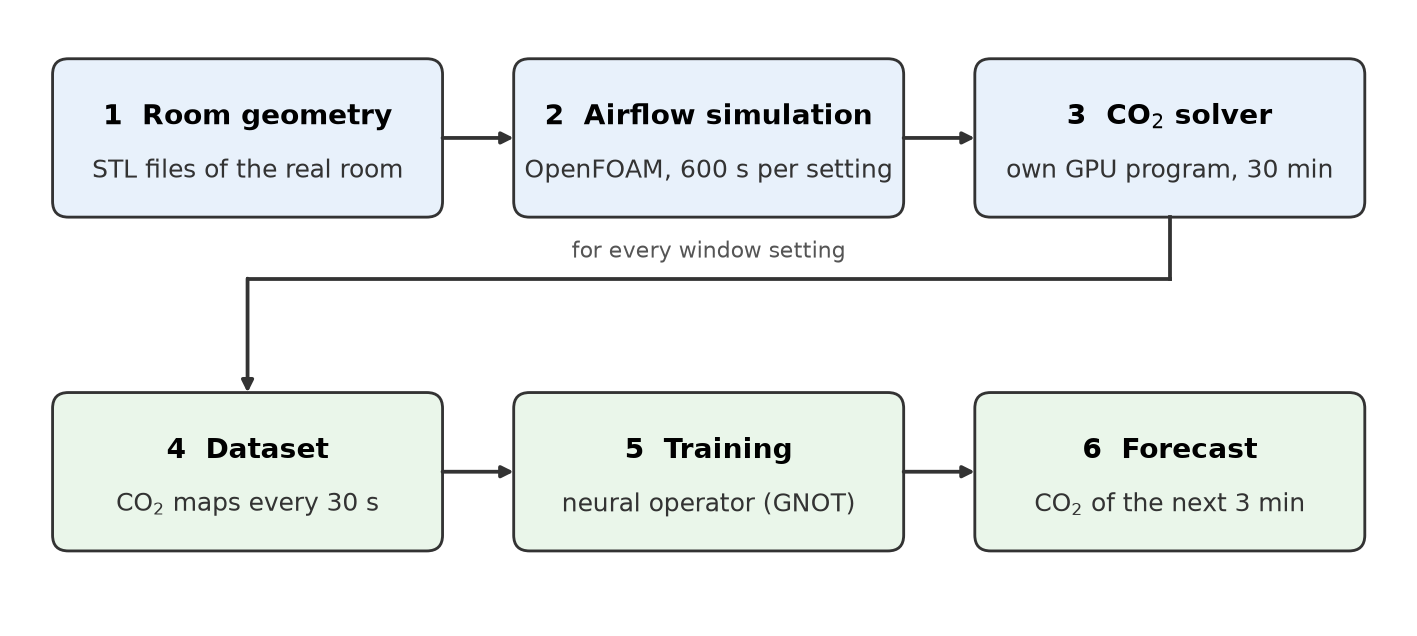
\includegraphics[width=\textwidth]{pipeline.png}
  \caption{Steps from the room to the forecast.}
  \label{fig:pipeline}
\end{figure}

I simulated the room in three steps. In the first setup the windows were opened in three groups and both
doors were open (39 scenarios). In the second setup only the windows W1, W3 and W6 can be opened and door~1 is
open (28 scenarios). Most results in this thesis are from this setup. In the third setup all 8 windows and
both doors can be open or closed. These 40 scenarios are running at the moment. \fref{fig:room} in
\cref{ch:room} shows where the windows and doors are.

\section{What I did}
\begin{itemize}
  \item I reproduced the results of \citet{bian2025} with their code and data.
  \item I built the complete chain from the room geometry to the trained model with open-source software.
  \item I wrote a \cotwo{} solver for the GPU that matches the \cotwo{} of OpenFOAM within about 2\,\%, and I
        found out how often the airflow has to be saved for this.
  \item I built the dataset a second time with this correction and compared the models trained on the old and
        on the new data.
  \item I started the simulations with all windows and doors.
  \item I tested faster simulations, a GPU solver and training without simulation data. These did not become
        part of the final method.
\end{itemize}

\section{Structure}
The thesis follows the order of the work. After the background in \cref{ch:background}, \cref{ch:repro}
shows the reproduction of the paper. \cref{ch:room} is about the room and the OpenFOAM simulations and
\cref{ch:dataset} about the \cotwo{} dataset. The model is described in \cref{ch:model} and its results in
\cref{ch:results}. \cref{ch:sensors} is about the sensor data, \cref{ch:notused} about the things I tested
and did not use, and \cref{ch:conclusion} is the conclusion.
